\chapter{シミュレーション結果}
Mathematicaを用いて,プレーナートラップ上に形成されるdcポテンシャルやrf擬ポテンシャルのシミュレーションを行った.その他,イオンの捕獲位置や永年周波数などの計算なども可能となっている.ここでは,各ポテンシャルの計算結果と永年周波数の計算方法について述べる.
\section{DCポテンシャル}
プレーナートラップの各電極を矩形電極となるように分割して,\Eq{rectangle_electrode}を用いることで,各dc電極が作る静電ポテンシャルの計算を行う.Mathematicaの計算を行うにあたり使用したプレーナートラップの電極モデルを\Fig{rect_electrode}に示す.

\begin{figure}[h]
	\begin{center}
		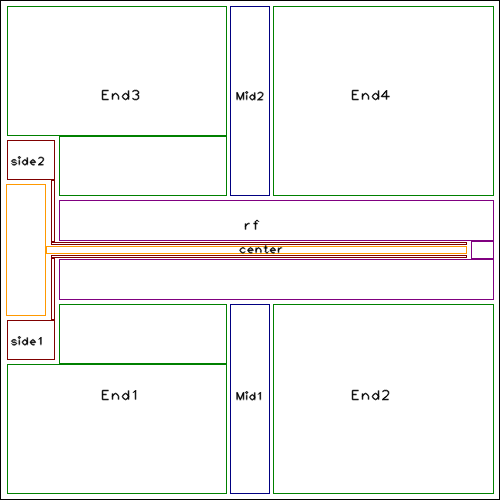
\includegraphics[width = 0.4\linewidth]{./simulation/figure/named_rect_electrode.png}
	\end{center}
	\caption{Mathematicaで計算する際に用いたプレーナートラップの電極モデル}
	\label{fig:rect_electrode}
\end{figure}

各dc電極によってプレーナートラップ上の点$(x,y,z)$に形成される静電ポテンシャル$\Phi_{\rm DC}(x,y,z)$は,分割した各矩形が$(x,y,z)$に形成する静電ポテンシャルの重ね合わせで
\large
\begin{align}
	\Phi_{\rm DC}(x,y,z) = \phi_{\rm End1} + \phi_{\rm End2} + \phi_{\rm End3} &+ \phi_{\rm End4} + \phi_{\rm Mid1} + \phi_{\rm Mid2} \notag \\
	&+ \phi_{\rm Side1} + \phi_{\rm Side2} + \phi_{\rm center},
\end{align}
\normalsize
と表すことができる.
%
\clearpage
%
\Fig{dc_potential}に\Tb{dc_set1}に示すdc電圧セットで計算したdcポテンシャルを示す.\Fig{dc_potential}は,z-y平面(x=0)(\Fig{z-y_x0})における計算結果となっている.
\begin{figure}[h]
			\begin{center}
				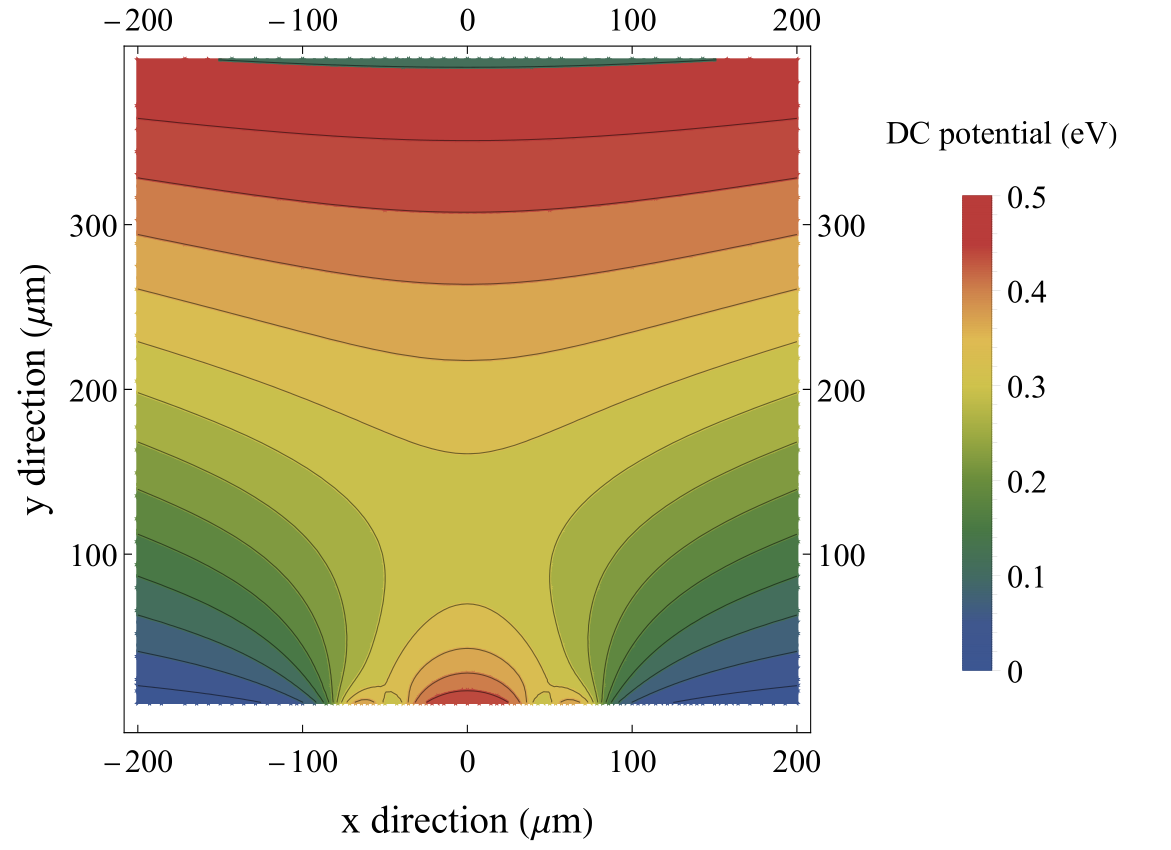
\includegraphics[width = 0.45\linewidth]{./simulation/figure/dc_potential_example.png}
					\caption{z-y平面(x=0)での\Tb{dc_set1}の条件で計算したdcポテンシャル}
					\label{fig:dc_potential}
			\end{center}
\end{figure}
\small
\begin{table}[h]
			\begin{center}
				\caption{シミュレーションで用いたdc電圧セット}
				\label{tab:dc_set1}
				\begin{tabular}{c|c} \hline \hline
					電極 & 印加電圧 (V) \\ \hline
					End1 & 1.41 \\ \hline
					End2 & 1.41 \\ \hline
					End3 & 1.41 \\ \hline
					End4 & 1.41 \\ \hline
					Mid1 & -1.532 \\ \hline
					Mid2 & -1.532 \\ \hline
					Side1 & 0.222 \\ \hline
					Side2 & 0.222 \\ \hline
					center & 0.225 \\ \hline
				\end{tabular}
			\end{center}
\end{table}
\normalsize
\begin{figure}[h]
	\begin{center}
		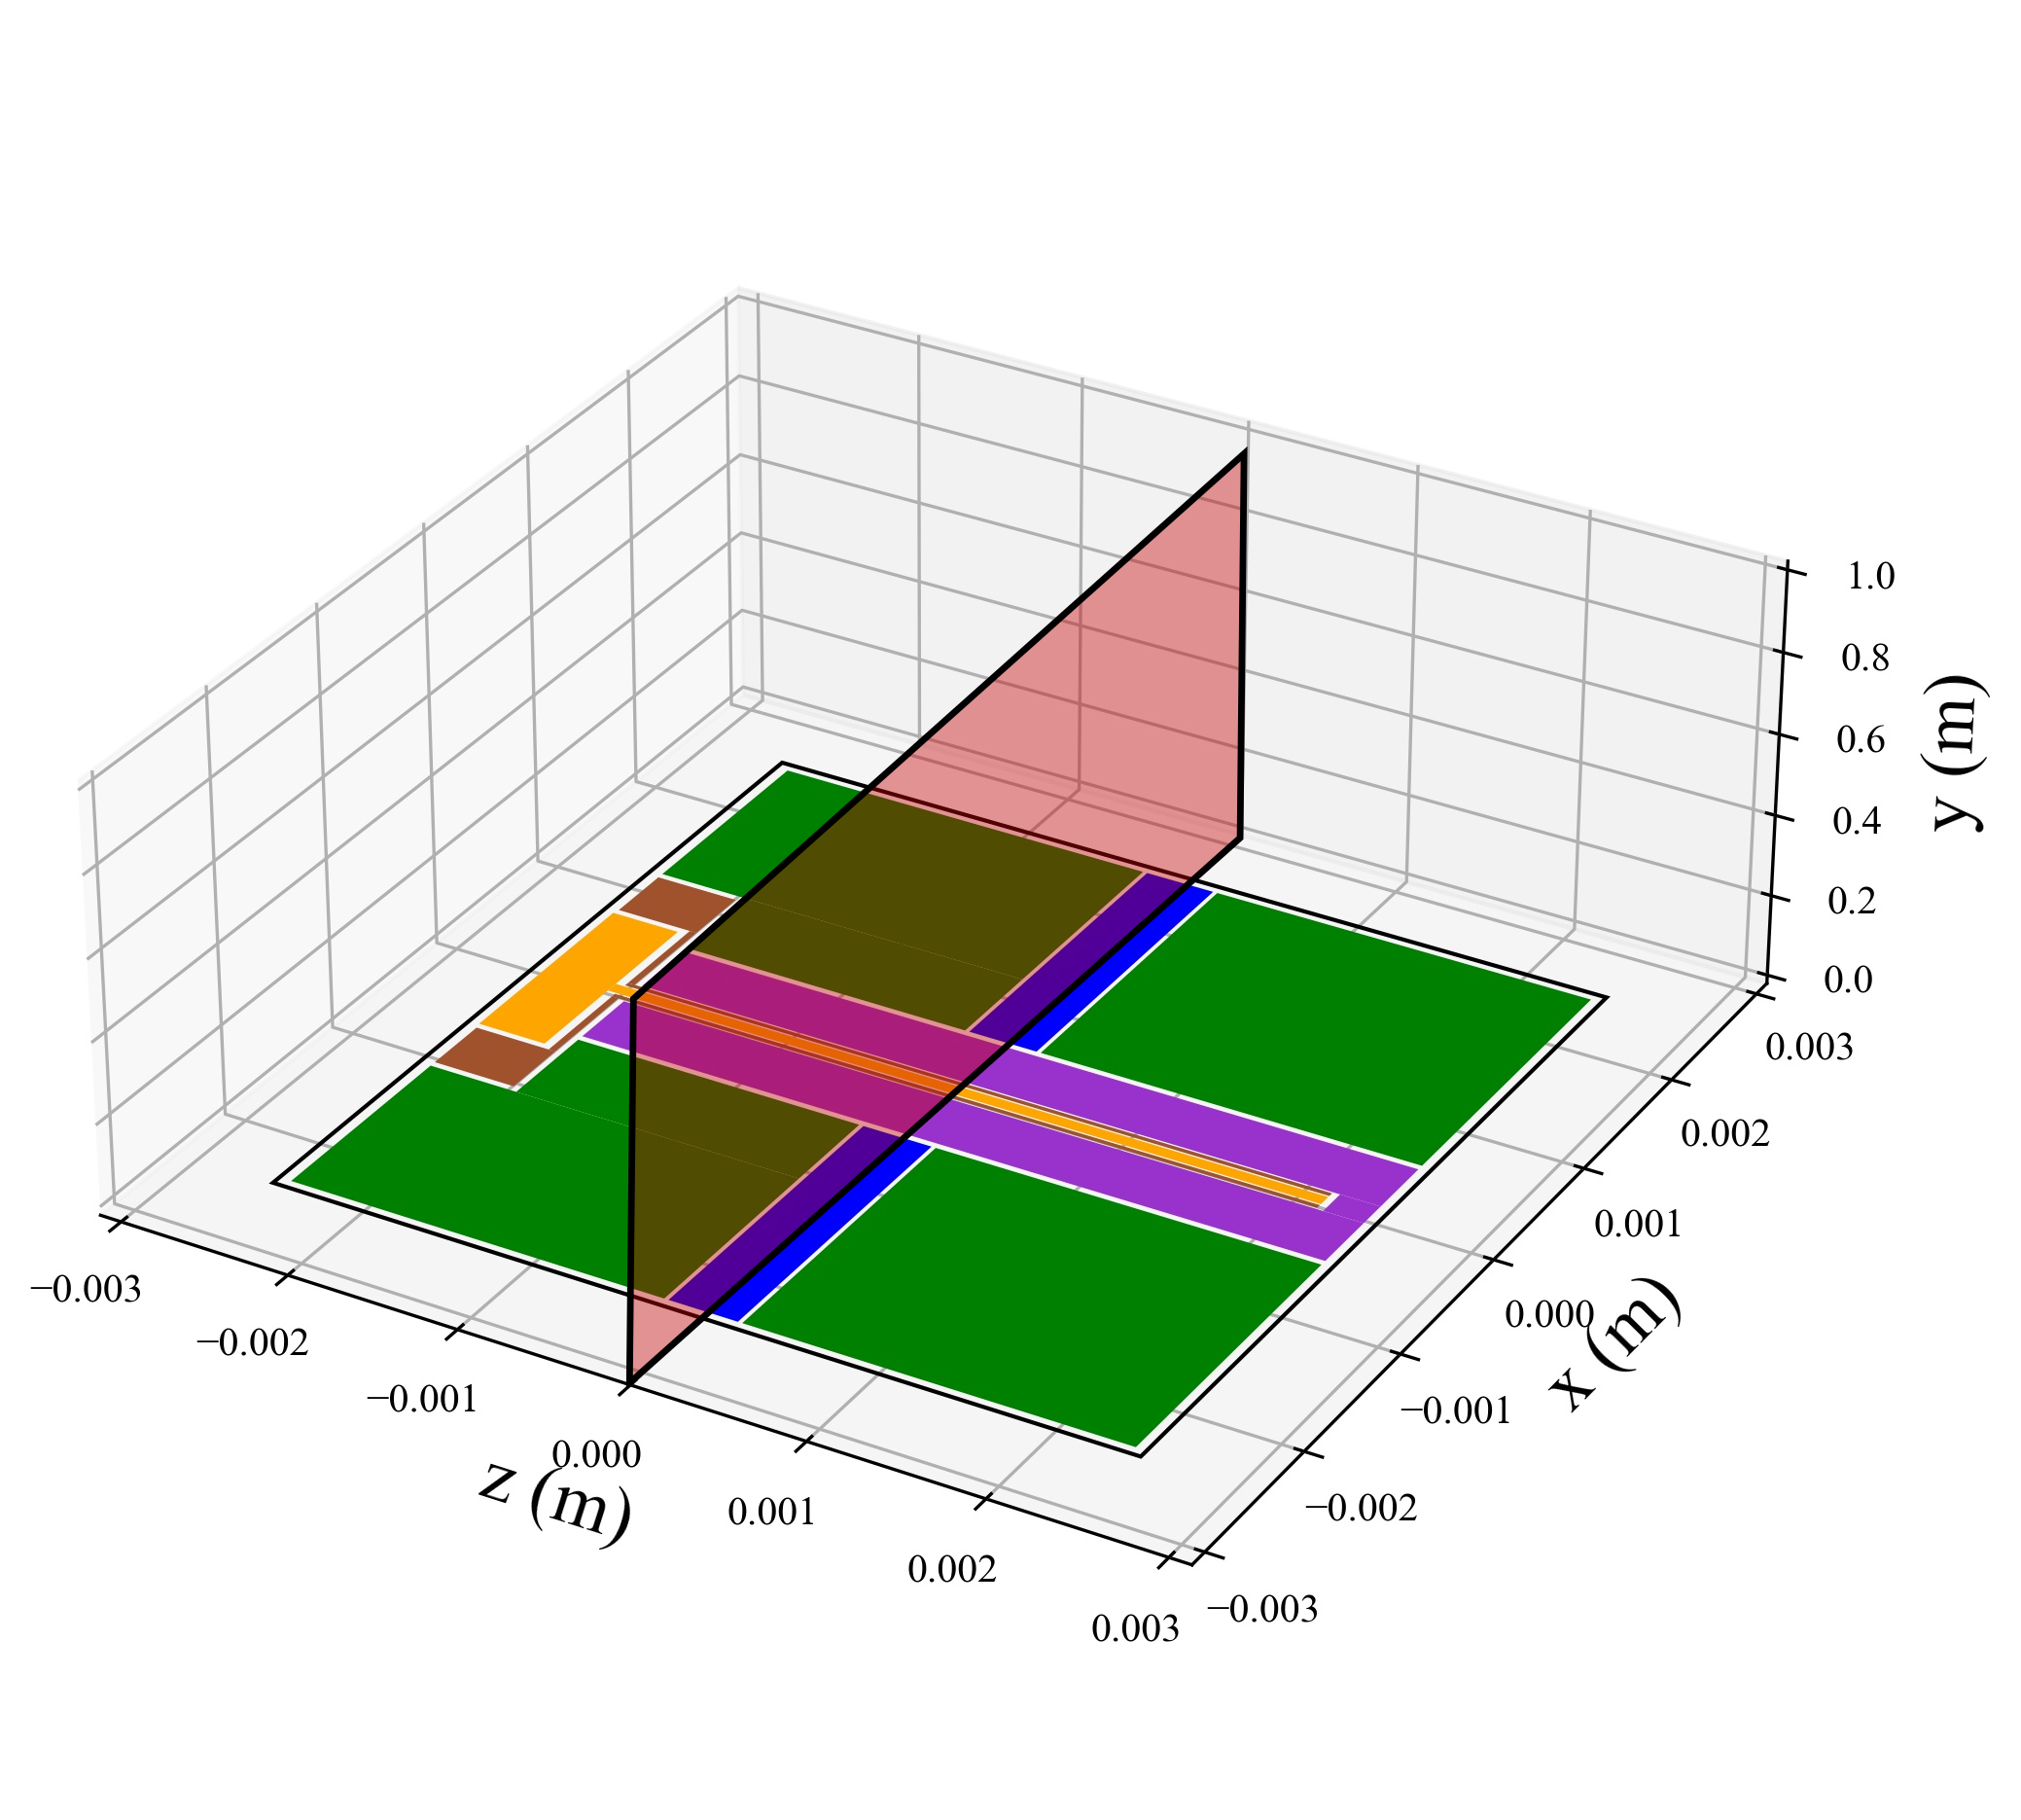
\includegraphics[width = 0.45\linewidth]{./simulation/figure/PlannarTrap_3D_z=0.png}
		\caption{プレーナートラップ上におけるz-y平面(x=0)}
		\label{fig:z-y_x0}
	\end{center}
\end{figure}
%
\clearpage
%

\section{rf擬ポテンシャル}
イオンのマイクロ運動の存在によって,イオンの永年運動に有効ポテンシャルがはたらく.したがって,シミュレーション上では振幅$V$のrf電圧が印加されたrf電極が任意の点につくる静電ポテンシャル$\phi (x,y,z)$を計算し,$\bm{E} = \nabla \phi$より電場を求め,\Eq{eff_pot}を用いて有効ポテンシャル$\Phi_{\rm eff}(x,y,z)$を計算する.ここでは一列配列イオンの捕獲を可能とするSingle-wellの条件と,二列配列イオンの捕獲を可能とするDouble-wellの条件におけるrf擬ポテンシャルの計算結果を示す.
\subsection{Single-wellにおけるrf擬ポテンシャル}
Single-wellの条件でのrf擬ポテンシャルについての計算結果を示す.\Fig{single-well_example_xy}にx-y平面(z=0)のrf擬ポテンシャルの計算結果を示す.このとき$\Omega_{\rm rf} = 27.2 \ {\rm MHz}, V_{\rm rf} = 62 \ {\rm V},R = 0.27$とした.
\begin{figure}[h]
	\begin{center}
	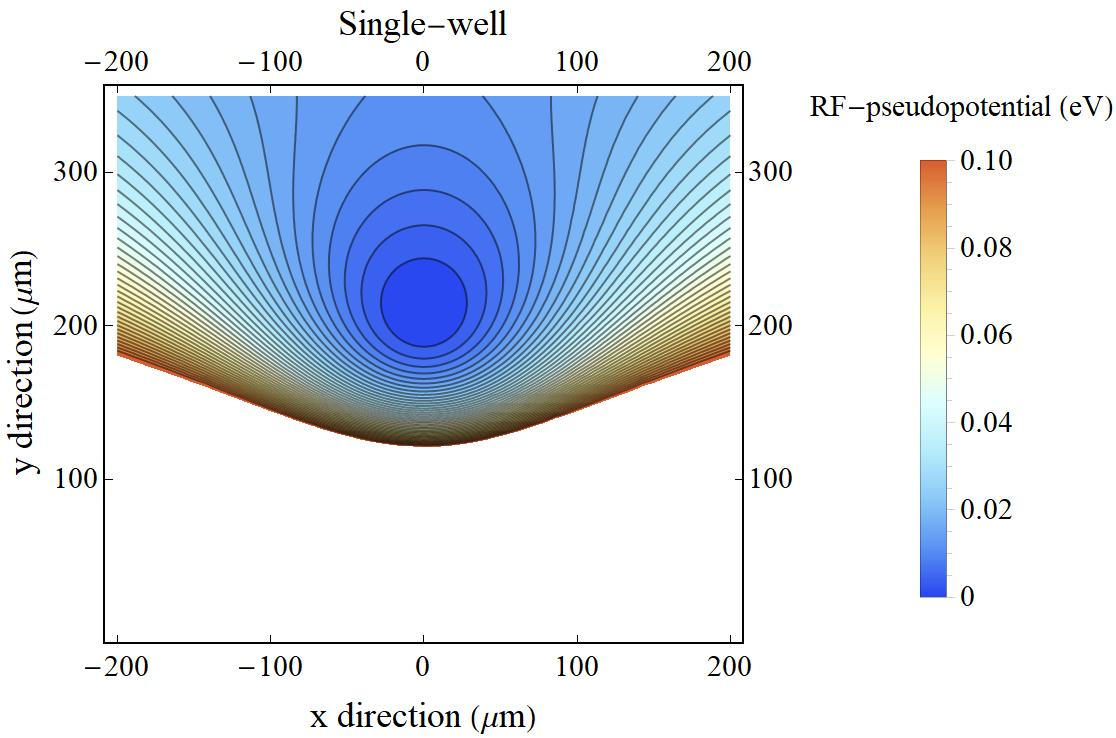
\includegraphics[width = 0.5\linewidth]{./simulation/figure/Single-well_Contour_xy@z=0.jpg}
	\caption{x-y平面(x=0)でのSingle-wellにおけるrf擬ポテンシャル}
	\label{fig:single-well_example_xy}
	\end{center}
\end{figure}
また,\Fig{single-well_example_zx}にz-x平面のrf擬ポテンシャルの様子を示す.\Fig{single-well_example_xy}において計算したrf擬ポテンシャルの最小値を取るトラップ表面からの高さ$y = 188.556 \ {\rm \mu m}$を用いている.
\begin{figure}[h]
	\begin{center}
	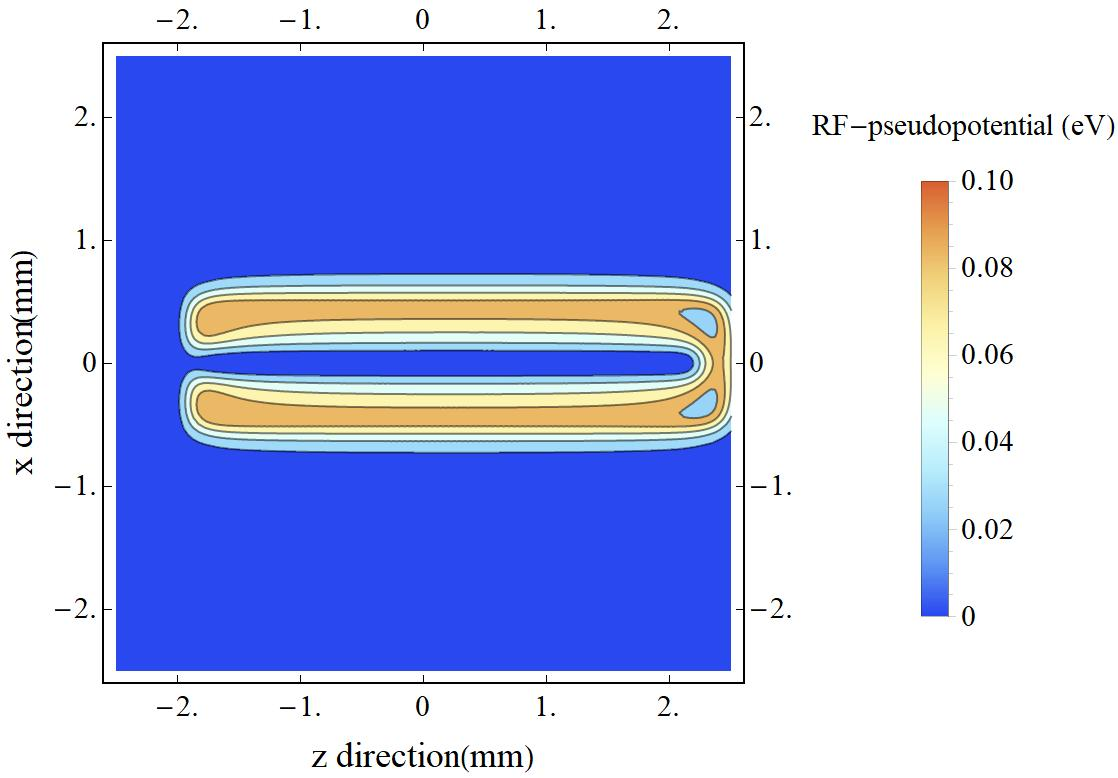
\includegraphics[width = 0.5\linewidth]{./simulation/figure/single-well_zx.jpg}
	\caption{z-x平面($y = 188.556 \ {\rm \mu m}$)でのSingle-wellにおけるrf擬ポテンシャル}
	\label{fig:single-well_example_zx}
	\end{center}
\end{figure}
\Fig{single-well_example_zx}より,rf擬ポテンシャルはz方向について閉じ込めのはたらきを持たないことが分かる.
\clearpage

\subsection{Double-wellにおけるrf擬ポテンシャル}
本実験で用いるプレーナートラップでは,rf電極に印加するrf電圧の振幅$V_{\rm rf}$とcenter-rf電極に印加するrf電圧の振幅$V_{\rm center-rf}$の比率
\large
\begin{align}
R = \frac{V_{\rm center-rf}}{V_{\rm rf}}
\end{align}
\normalsize
を制御することでイオンを二列に配列させることが可能になっている.

\Fig{R075}$\sim$\Fig{R100}に異なるRの値に対するrf擬ポテンシャルの変化の様子を示す.
\begin{figure}[h]
	\begin{minipage}{0.48\linewidth}
		\begin{center}
			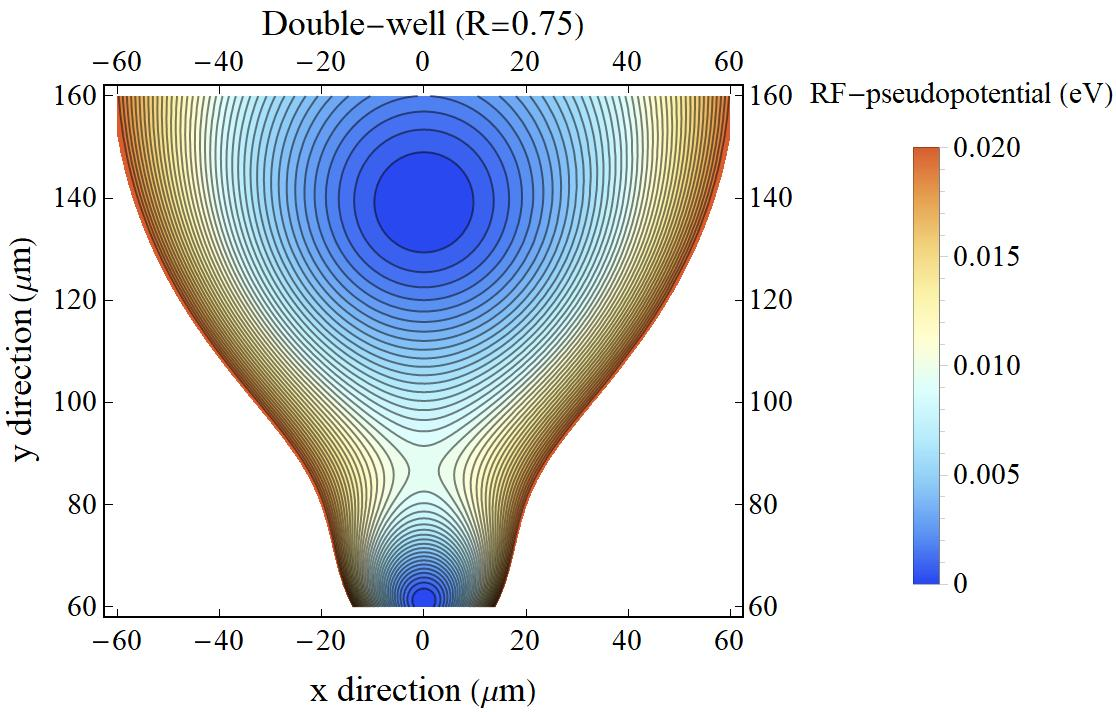
\includegraphics[width = 0.9\columnwidth]{./simulation/figure/rf_pseudopotential_R=075.jpg}
			\caption{$R=0.75$}
			\label{fig:R075}
		\end{center}
	\end{minipage}
	\begin{minipage}{0.48\linewidth}
			\begin{center}
				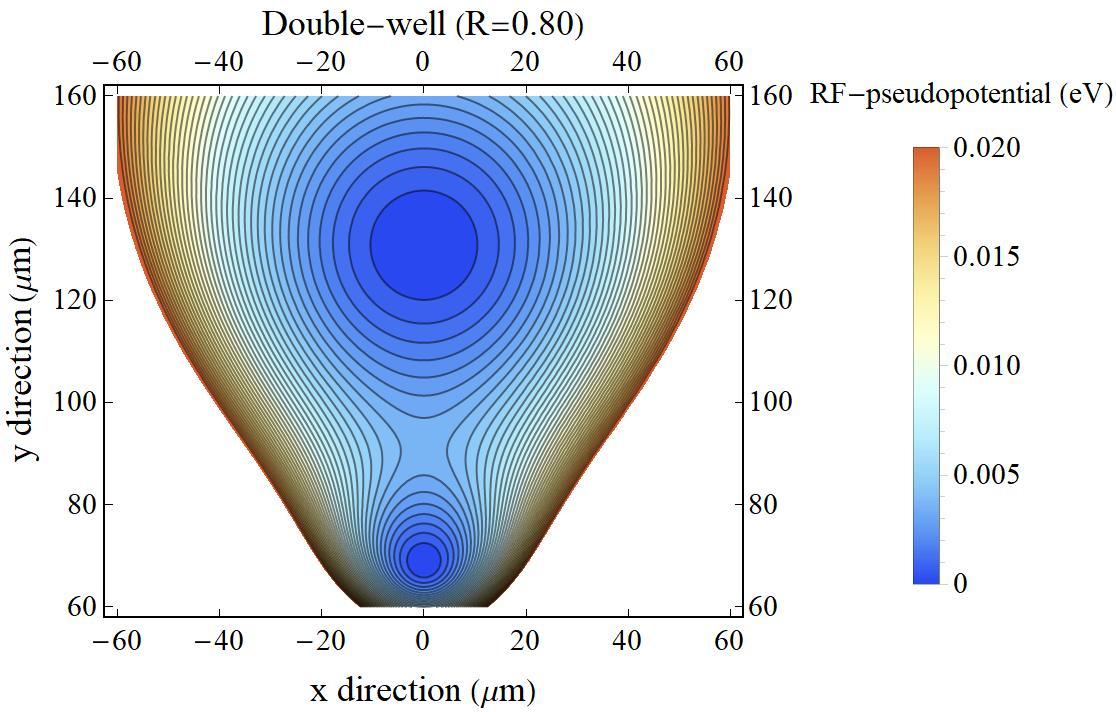
\includegraphics[width = 0.9\columnwidth]{./simulation/figure/rf_pseudopotential_R=080.jpg}
				\caption{$R=0.80$}
				\label{fig:R080}
			\end{center}
		\end{minipage}
\end{figure}
\begin{figure}[h]
	\begin{minipage}{0.48\linewidth}
		\begin{center}
			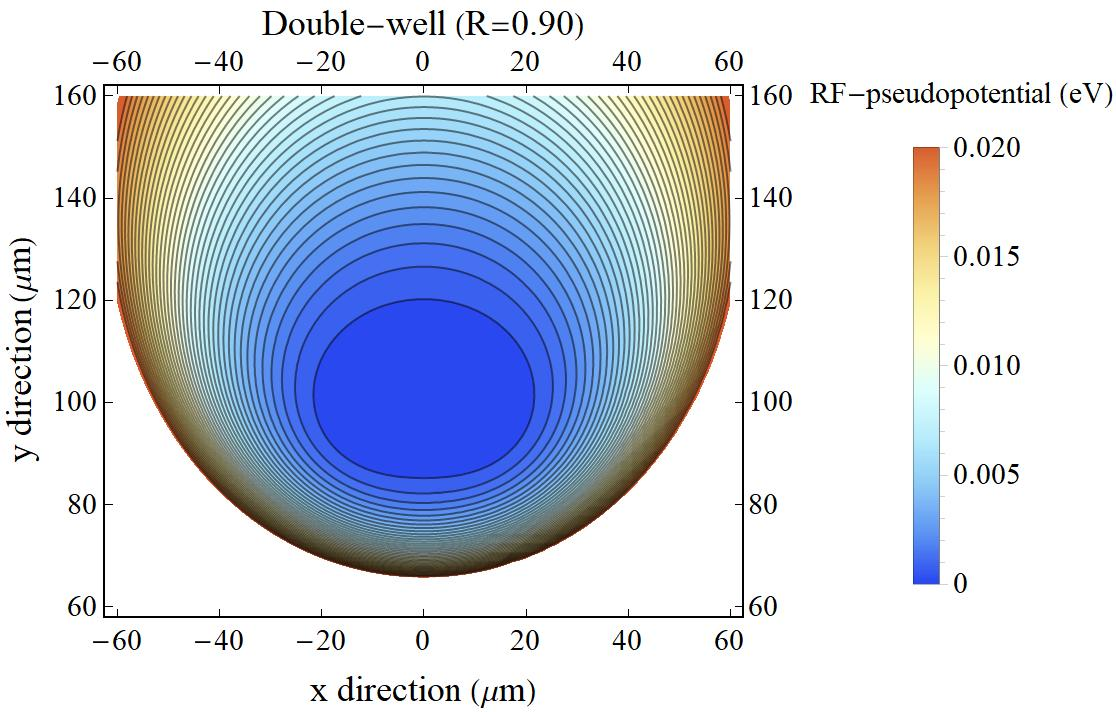
\includegraphics[width = 0.9\columnwidth]{./simulation/figure/rf_pseudopotential_R=090.jpg}
			\caption{$R=0.90$}
			\label{fig:R090}
		\end{center}
	\end{minipage}
	\begin{minipage}{0.48\linewidth}
			\begin{center}
				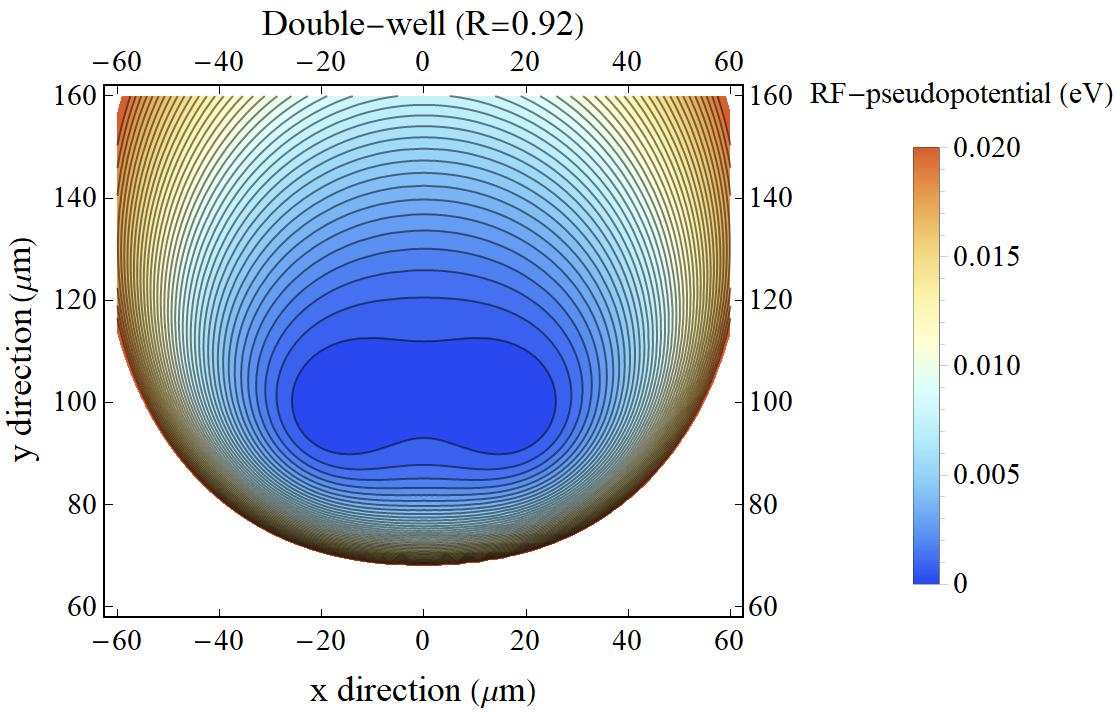
\includegraphics[width = 0.9\columnwidth]{./simulation/figure/rf_pseudopotential_R=092.jpg}
				\caption{$R=0.92$}
				\label{fig:R092}
			\end{center}
		\end{minipage}
\end{figure}
\begin{figure}[h]
	\begin{minipage}{0.48\linewidth}
		\begin{center}
			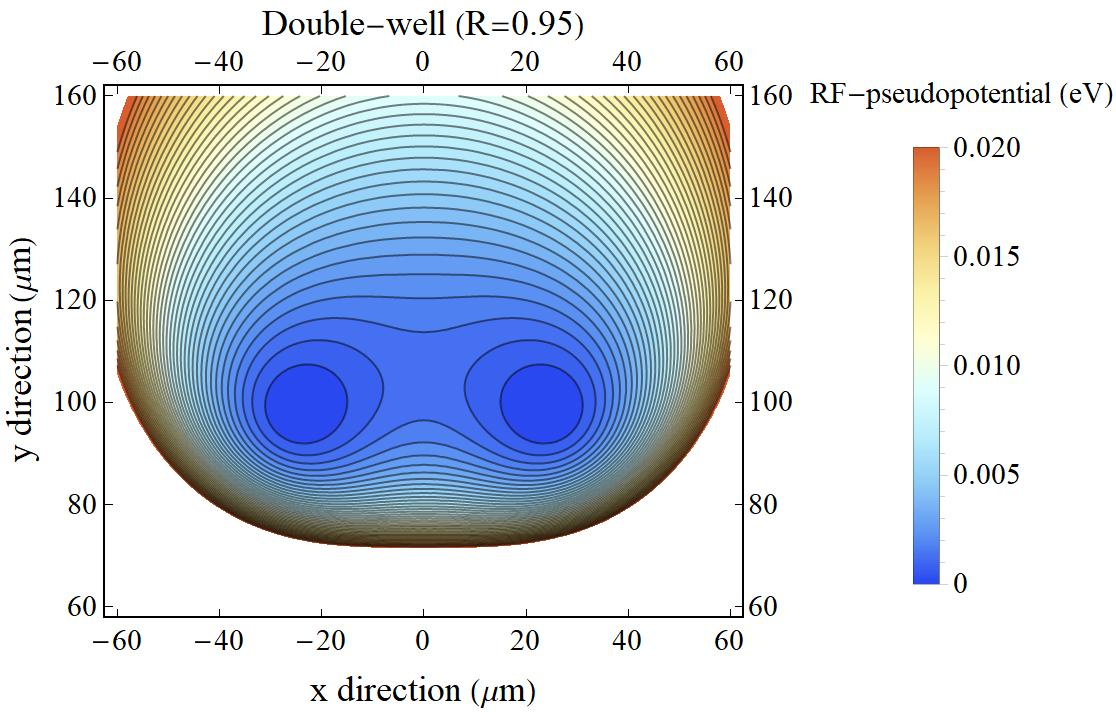
\includegraphics[width = 0.9\columnwidth]{./simulation/figure/rf_pseudopotential_R=095.jpg}
			\caption{R=0.95}
			\label{fig:R095}
		\end{center}
	\end{minipage}
	\begin{minipage}{0.48\linewidth}
			\begin{center}
				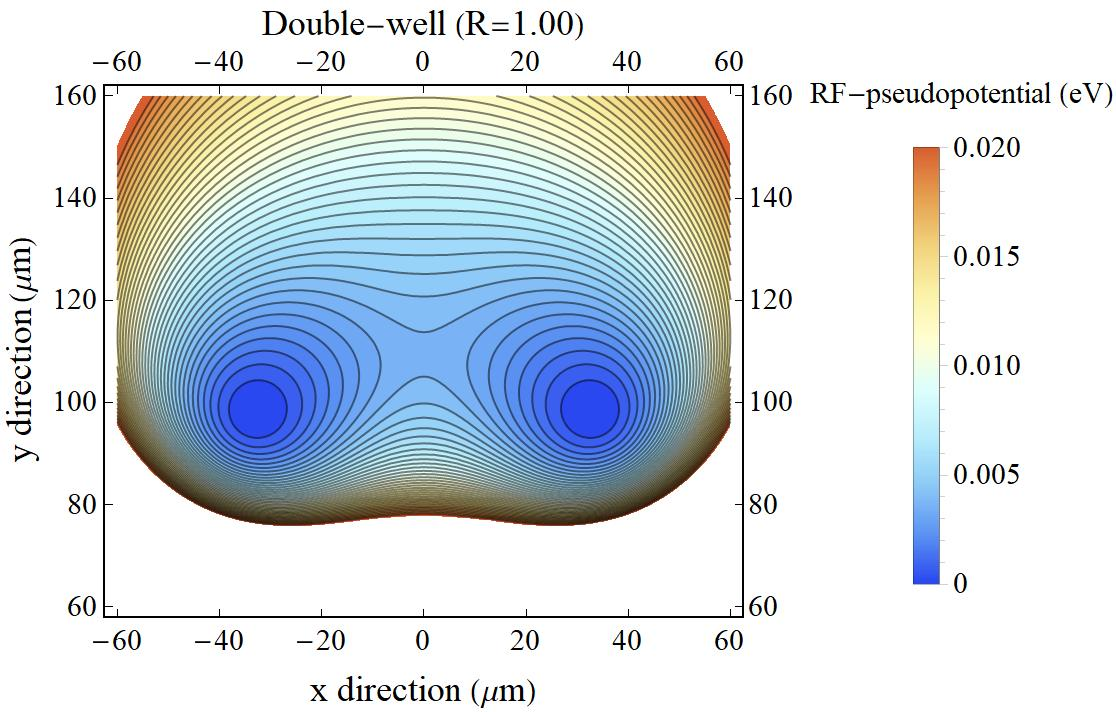
\includegraphics[width = 0.9\columnwidth]{./simulation/figure/rf_pseudopotential_R=100.jpg}
				\caption{$R=1.0$}
				\label{fig:R100}
			\end{center}
		\end{minipage}
\end{figure}

\clearpage

\section{Secularポテンシャル}
イオンを捕獲するときのトラップポテンシャルは,dcポテンシャルとrf擬ポテンシャルの重ね合わせ,
\large
\begin{align}
	\Phi_{\rm secular} = \Phi_{\rm DC} + \Phi_{\rm eff}
\end{align}
\normalsize
で表される.これをSecularポテンシャルと呼ぶ.\Fig{SecPot_single-well}にSingle-wellの条件におけるSecularポテンシャルを示す.

\begin{figure}[h]
	\begin{center}
		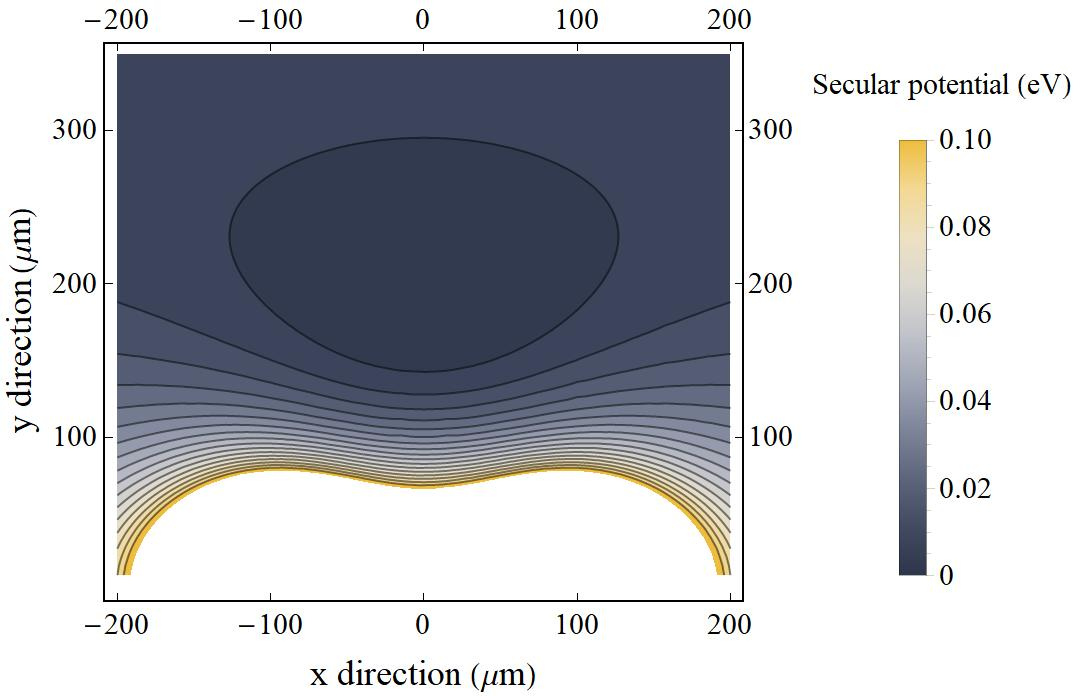
\includegraphics[width = 0.6\linewidth]{./simulation/figure/Single-well_Secular_pot_xy.jpg}
		\caption{x-y平面でのSingle-wellの条件におけるSecularポテンシャル}
		\label{fig:SecPot_single-well}
	\end{center}
\end{figure}

次に,\Fig{SecPot_double-well}にDouble-wellの条件におけるSecularポテンシャルを示す.

\begin{figure}[h]
	\begin{center}
		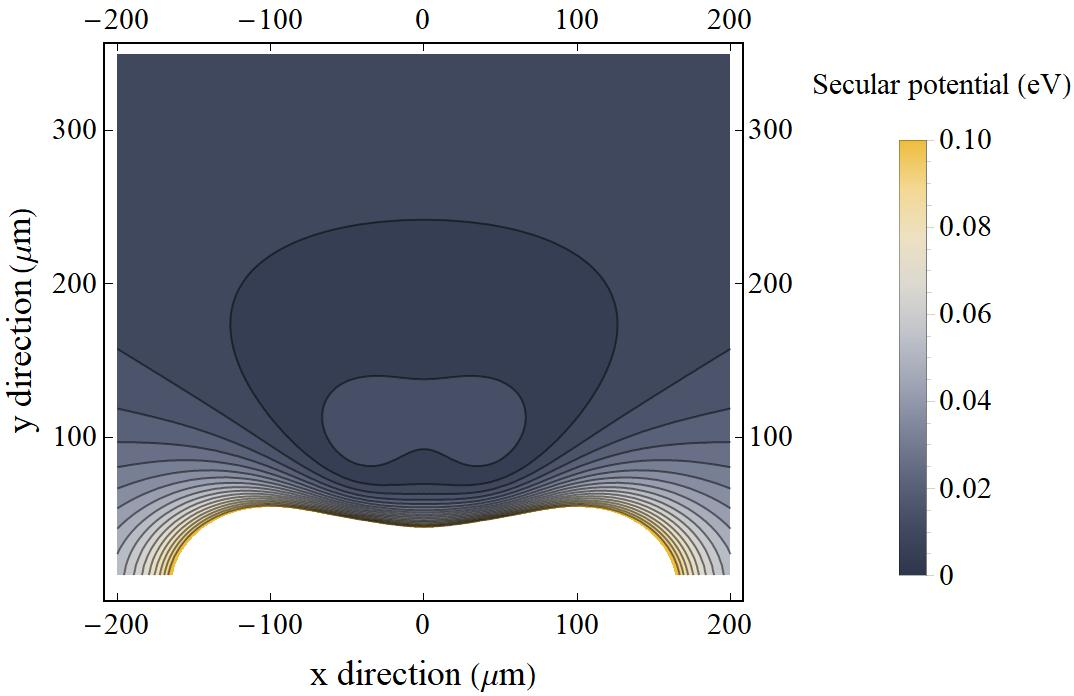
\includegraphics[width = 0.6\linewidth]{./simulation/figure/Double-well_Secular_pot_xy.jpg}
		\caption{x-y平面でのDouble-wellの条件におけるSecularポテンシャル}
		\label{fig:SecPot_double-well}
	\end{center}
\end{figure}

%
\clearpage
%
ここで,\Fig{Double-well_z0}に\Fig{SecPot_double-well}で求められたy方向に関するSecularポテンシャルの極小値を用いて,z=0でのx方向におけるSecularポテンシャルの概形を示す.
\begin{figure}[h]
	\begin{center}
		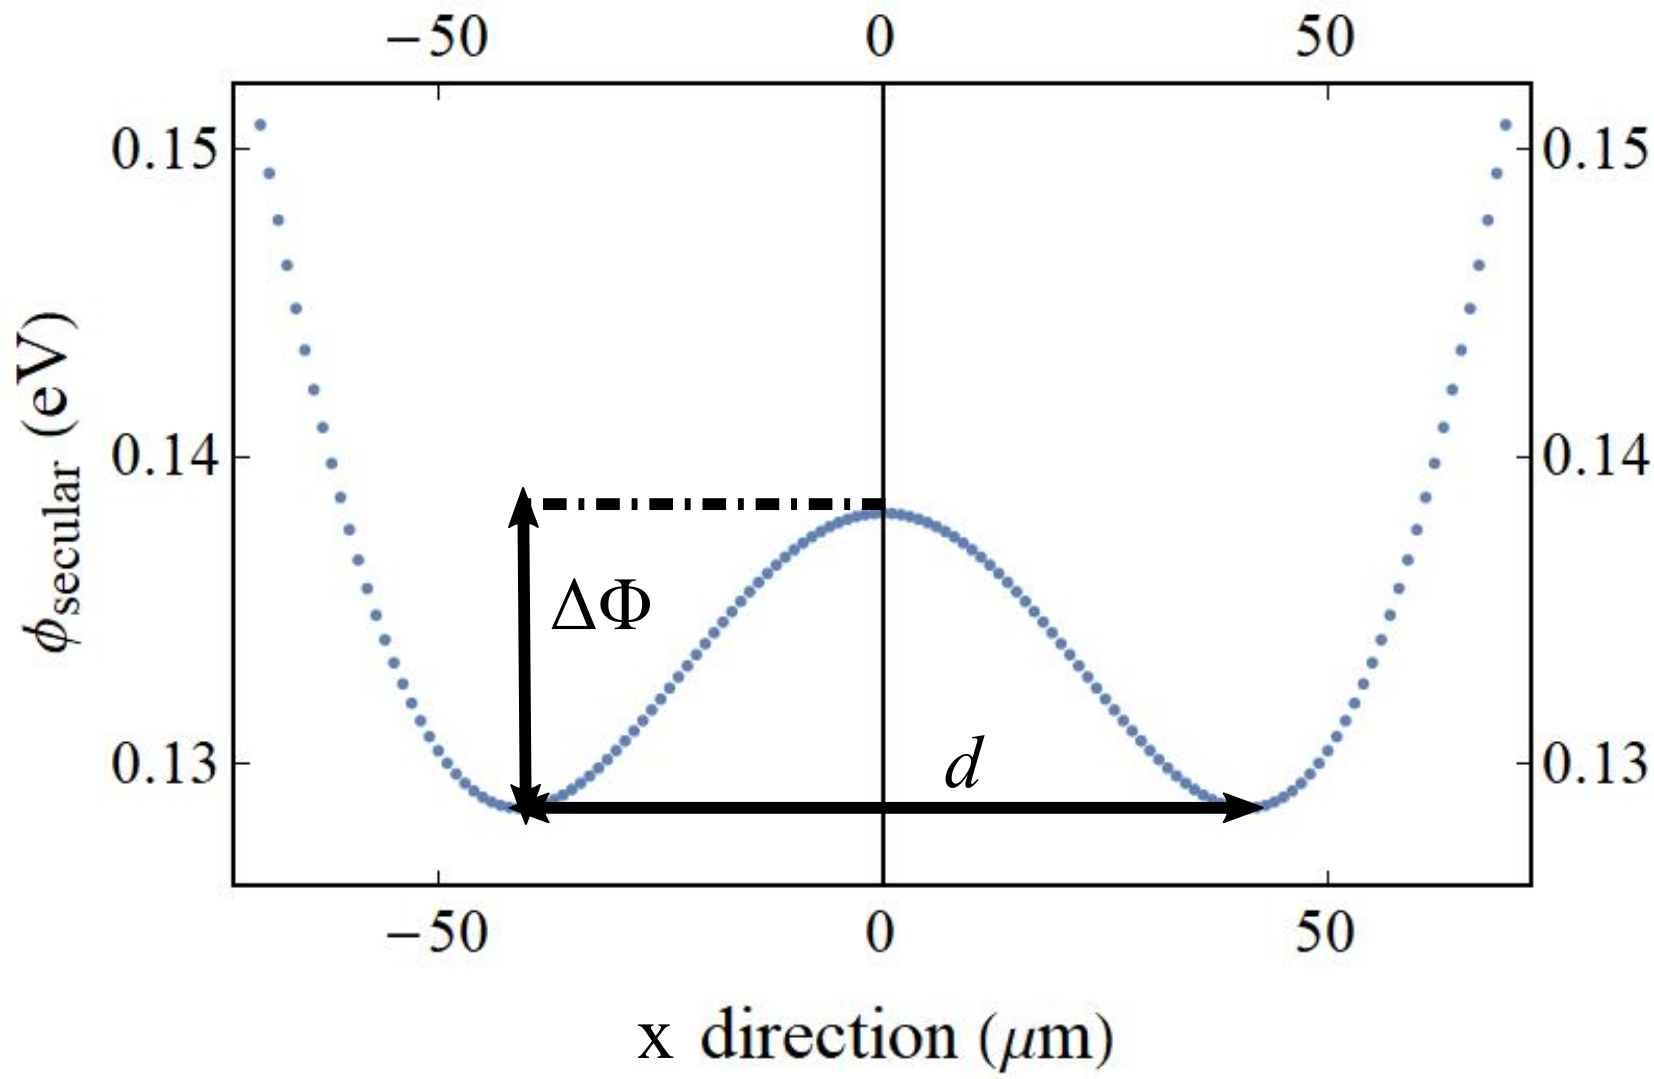
\includegraphics[width = 0.6\linewidth]{./simulation/figure/Double-well_z=0.png}
		\caption{Double-wellの条件におけるSecularポテンシャルのy方向の極小値におけるx軸に関するSecularポテンシャル(z=0)}
		\label{fig:Double-well_z0}
	\end{center}
\end{figure}

シミュレーションにおいて,Double-wellの条件でイオン列間距離$d$とイオン列間に生じる電位障壁$\Delta \Phi$の$R$特性を調べた.$R$と$\Delta \Phi$は\Fig{Double-well_z0}に示すように定めた.得られた$R$ - $d$特性および$R$ - $\Delta \Phi$特性を\Fig{calc_R-d}と\Fig{calc_R-phi}に示す.

\begin{figure}[h]
	\begin{minipage}{0.5\linewidth}
		\begin{center}
			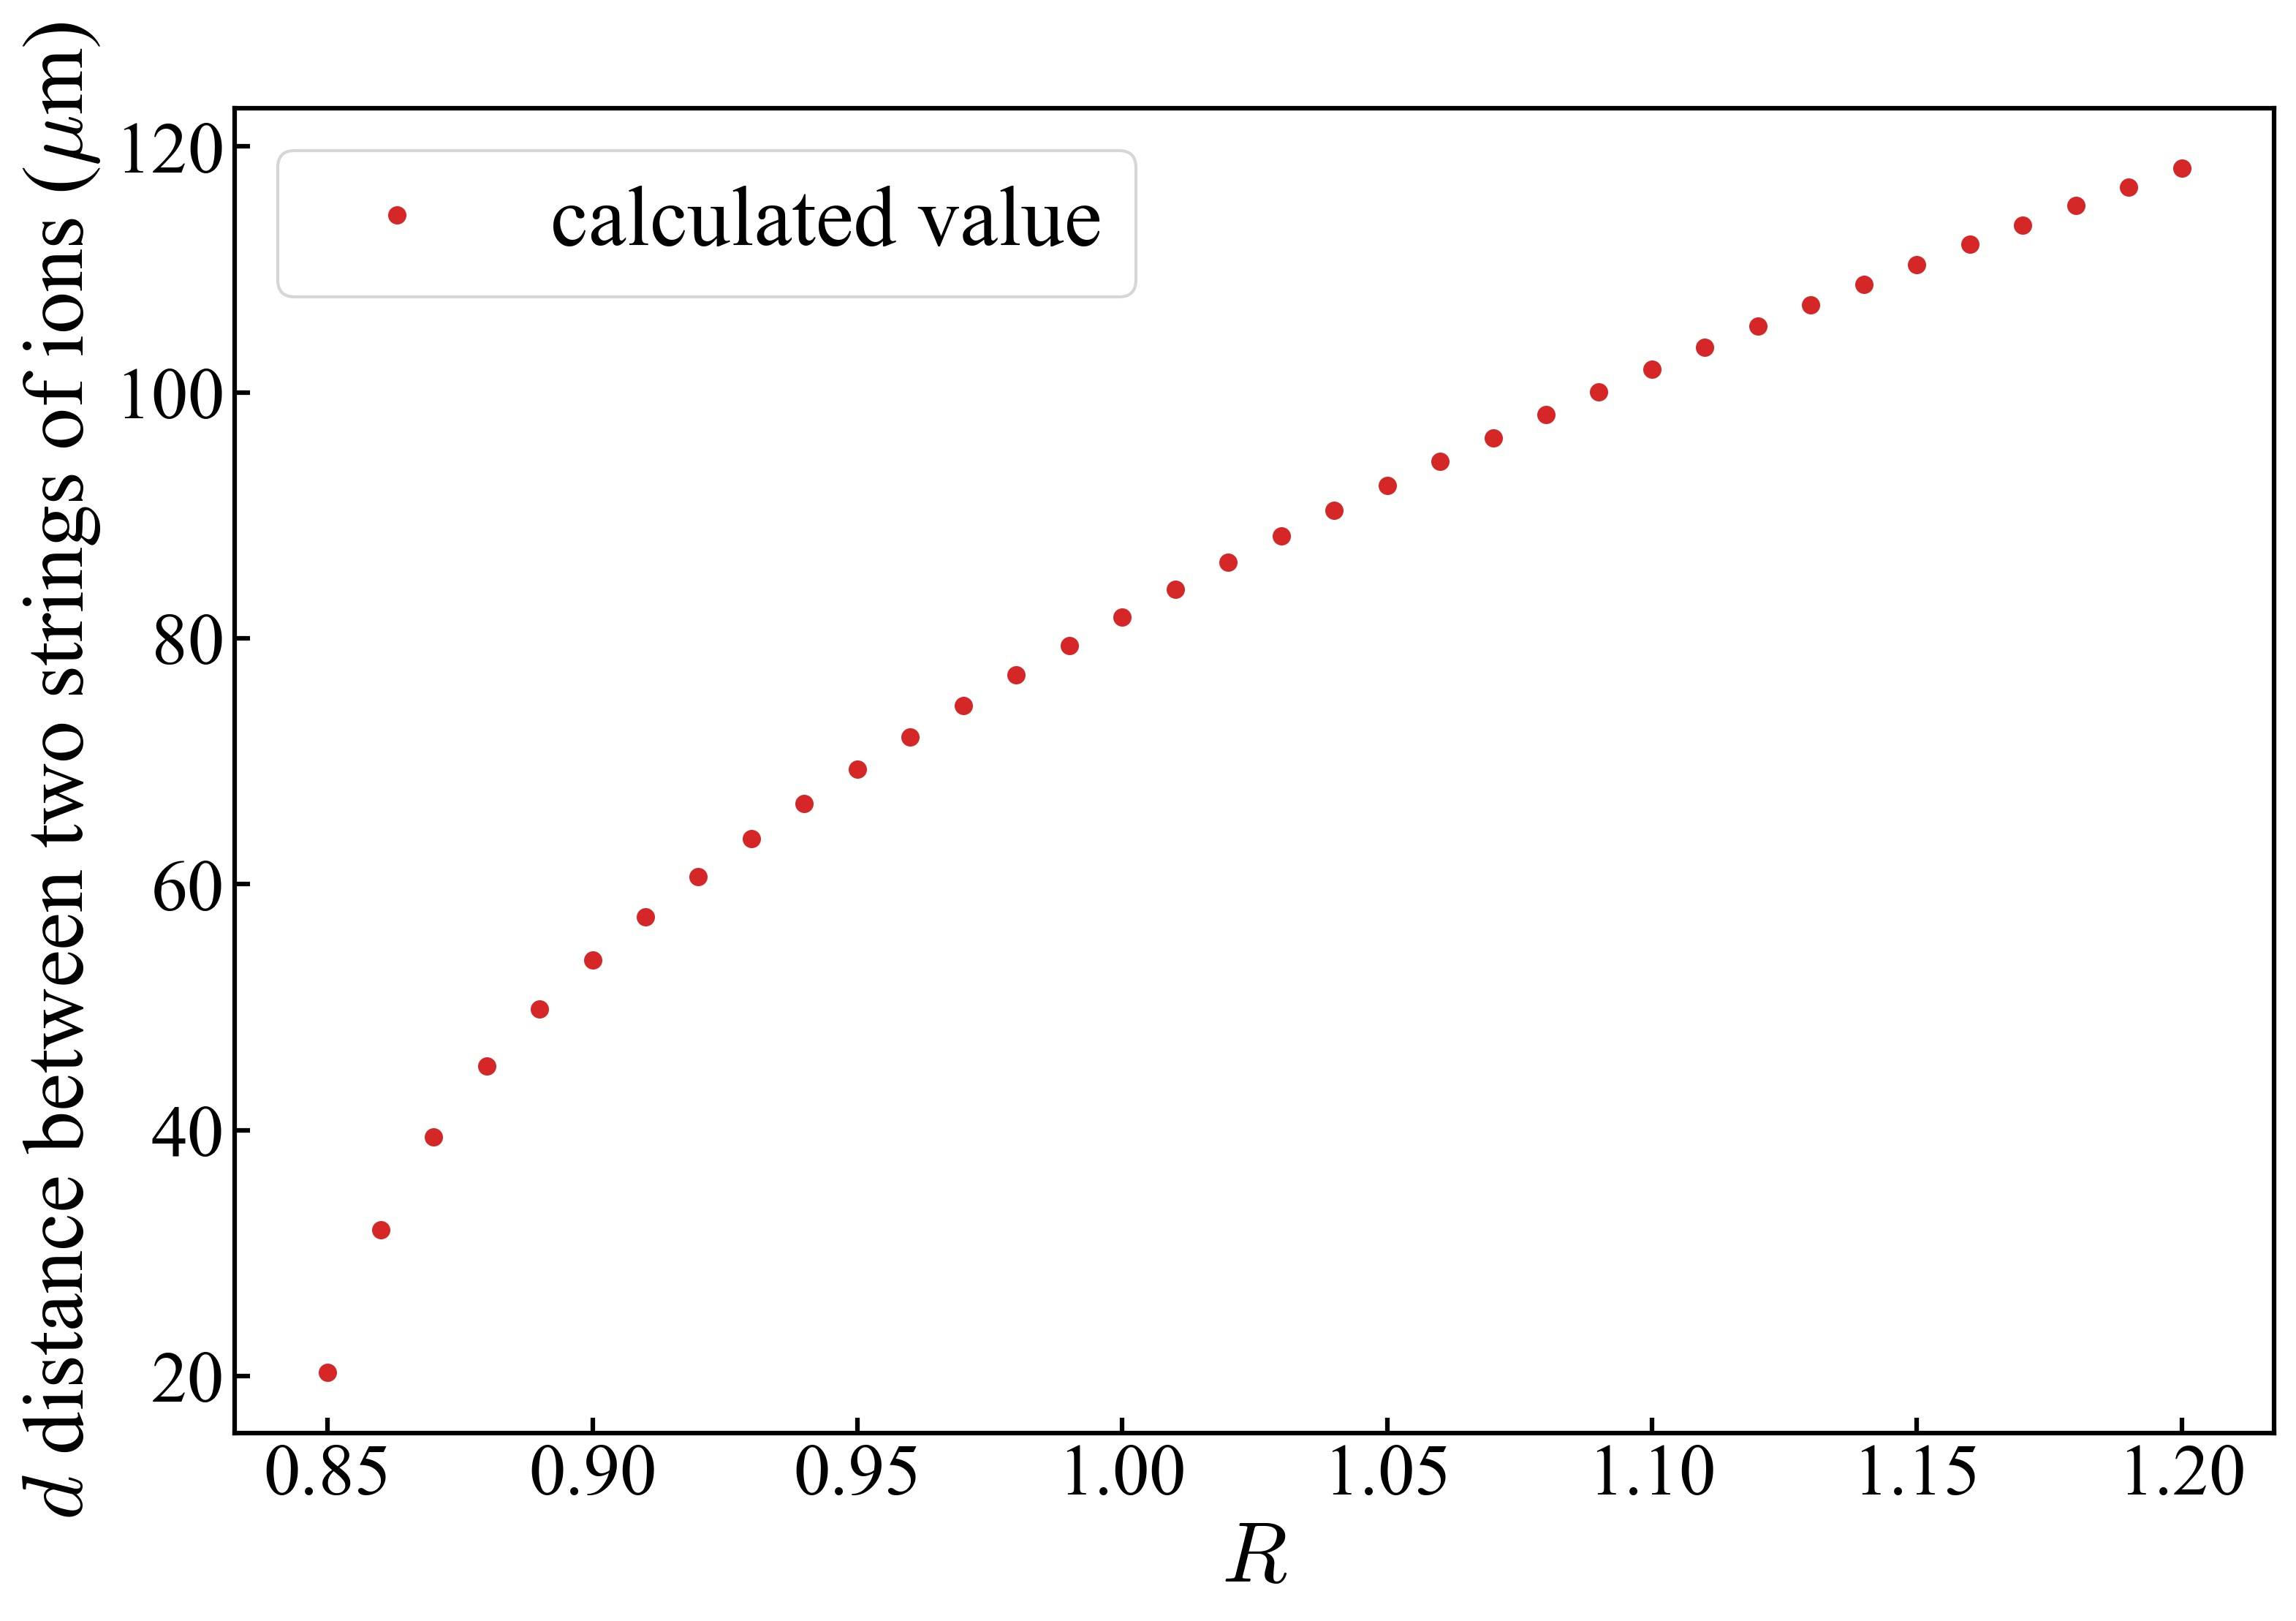
\includegraphics[width = 0.98\columnwidth]{./simulation/figure/Calc_R_d.jpg}
			\caption{$R$ - $d$特性のシミュレーション結果}
			\label{fig:calc_R-d}
		\end{center}
	\end{minipage}
	\begin{minipage}{0.5\linewidth}
		\begin{center}
			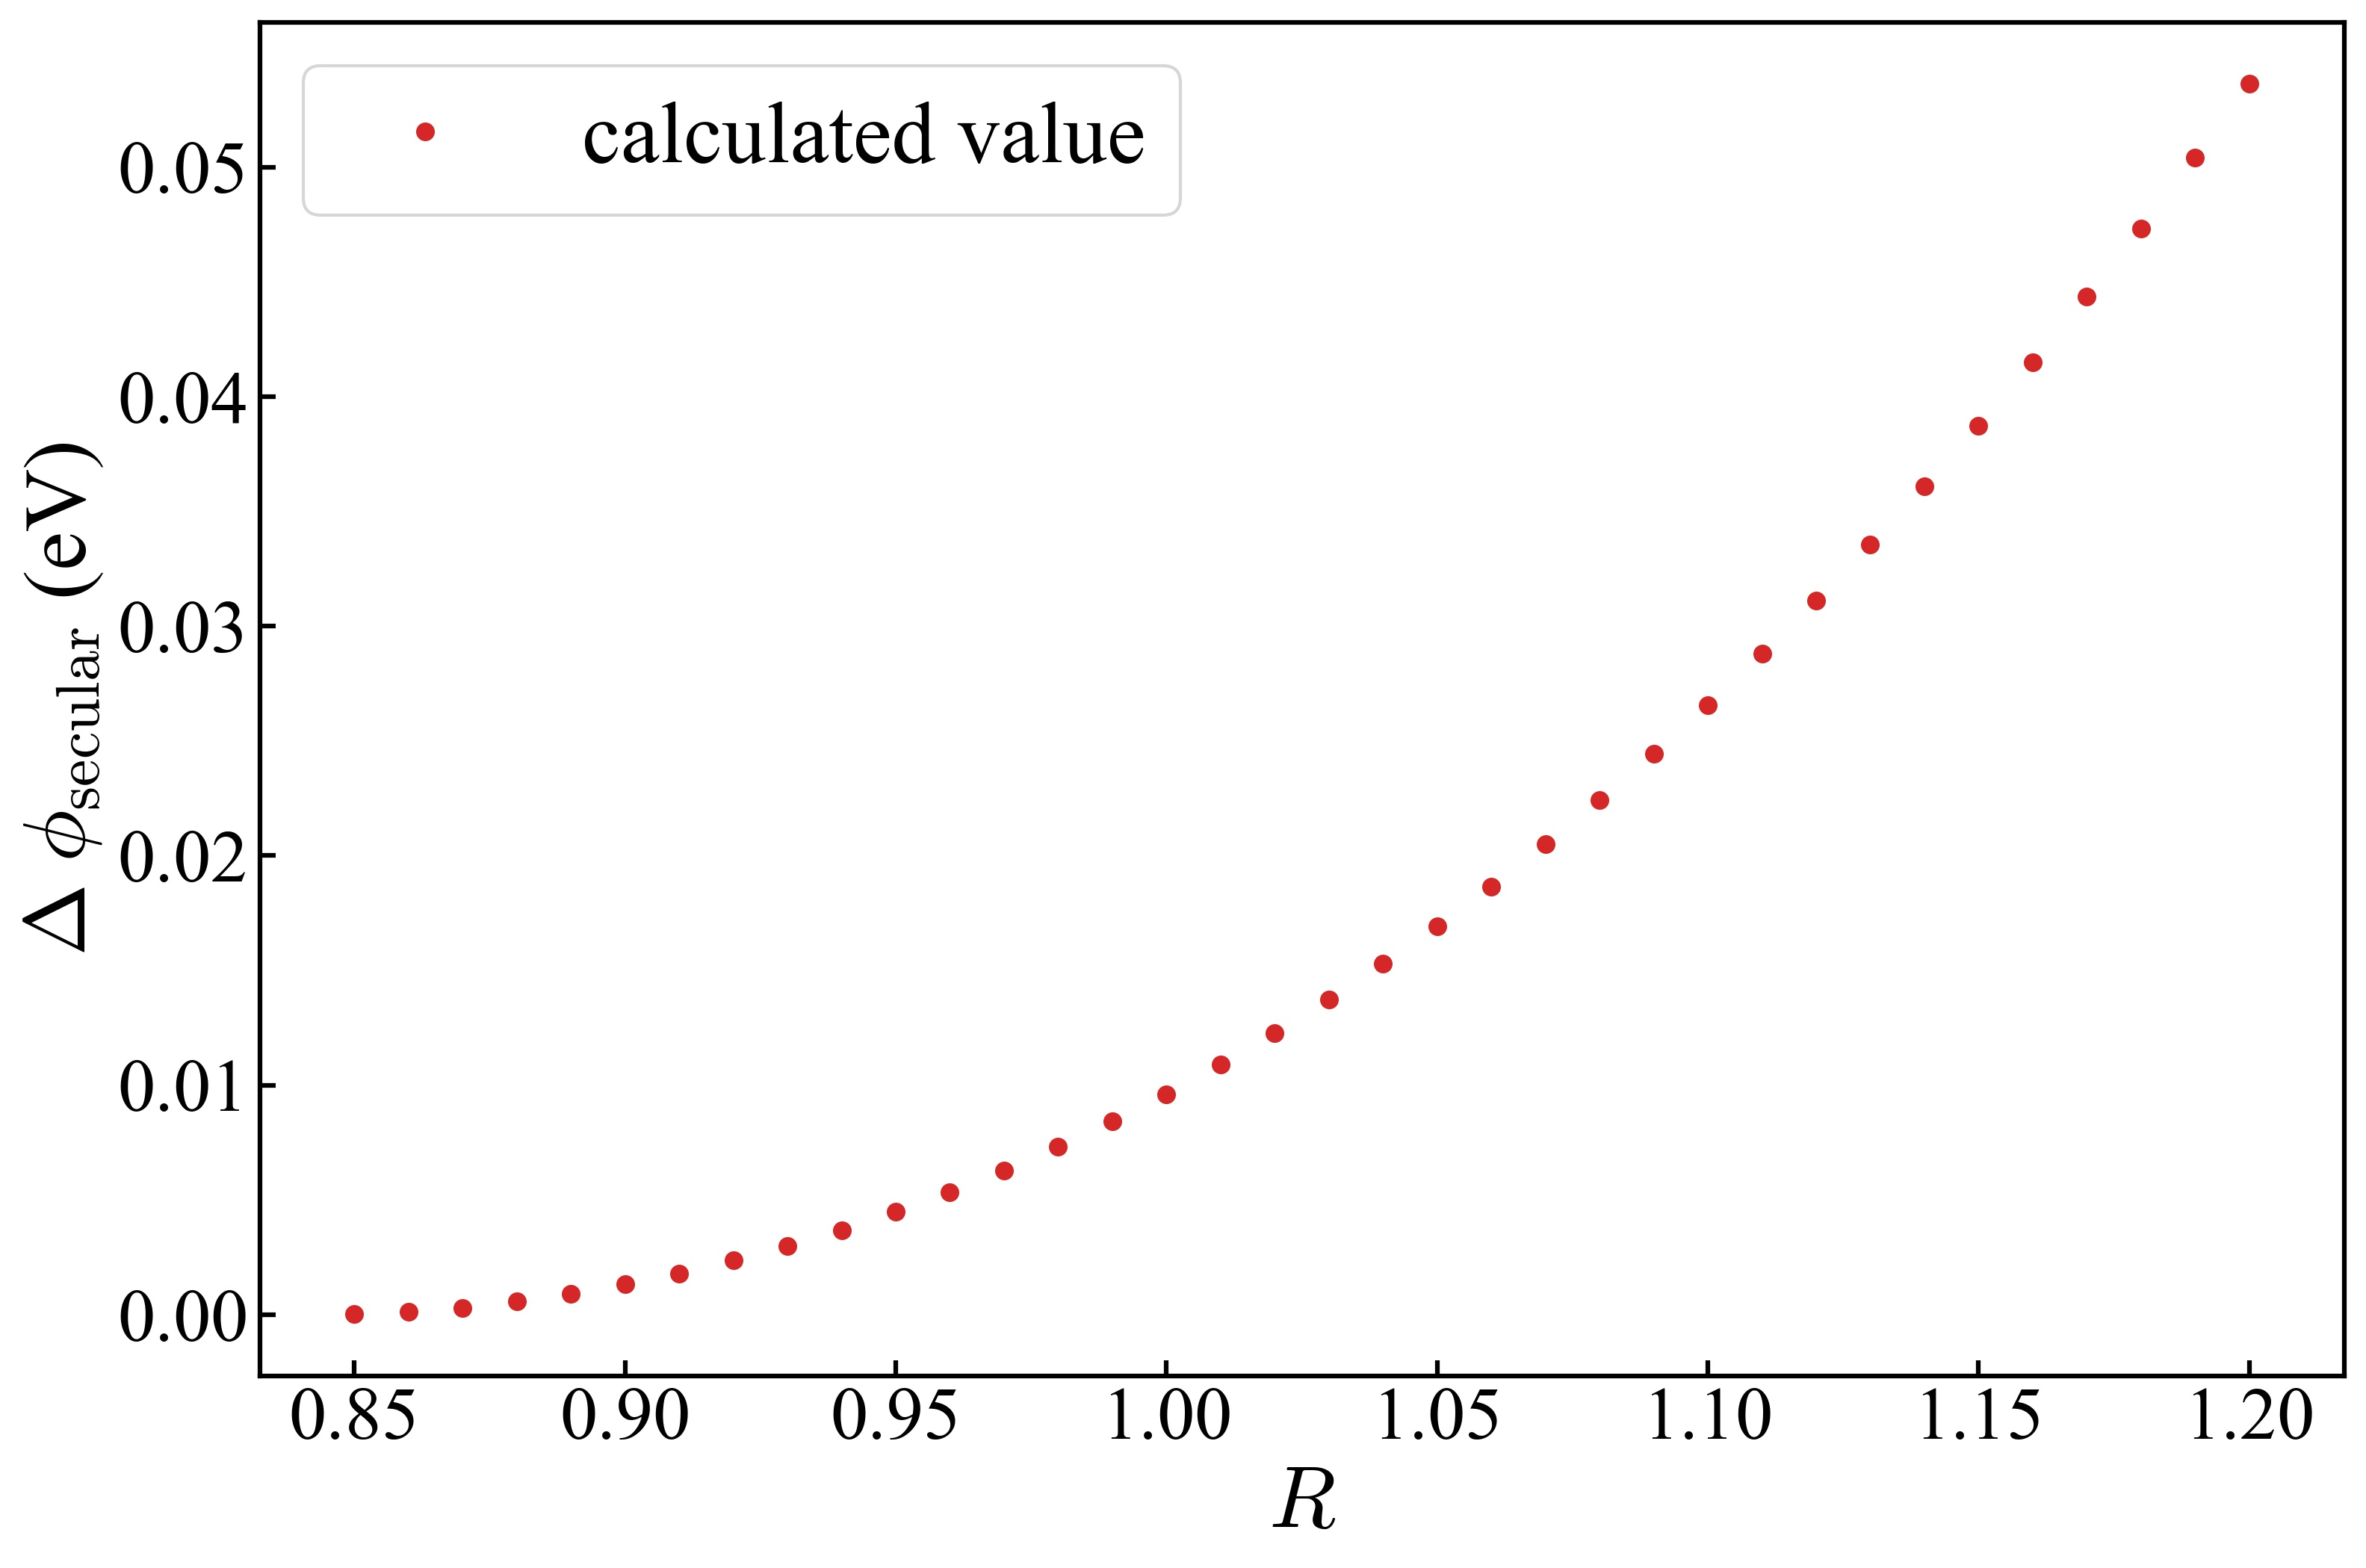
\includegraphics[width = 0.98\columnwidth]{./simulation/figure/Calc_R_phi.jpg}
			\caption{$R$ - $\Delta \phi$特性のシミュレーション結果}
			\label{fig:calc_R-phi}
		\end{center}
	\end{minipage}
\end{figure}
これより,$R$の値を大きくしてくと,イオン列間距離$d$は広がり,また,電位障壁$\Delta \Phi$が高くなっていくことが分かる.

%
\clearpage
%
\section{永年周波数の計算方法}
シミュレーション上で各方向での永年周波数の計算を可能としている.ここではSingle-wellの条件にてz軸方向の永年周波数を例に挙げて,永年周波数の計算方法について述べる.\Fig{determine_SecFreq}に,計算して求められたy方向の極小値を用いて,x=0でのz方向に関するSecularポテンシャルの概形を示す.
\begin{figure}[h]
	\begin{center}
		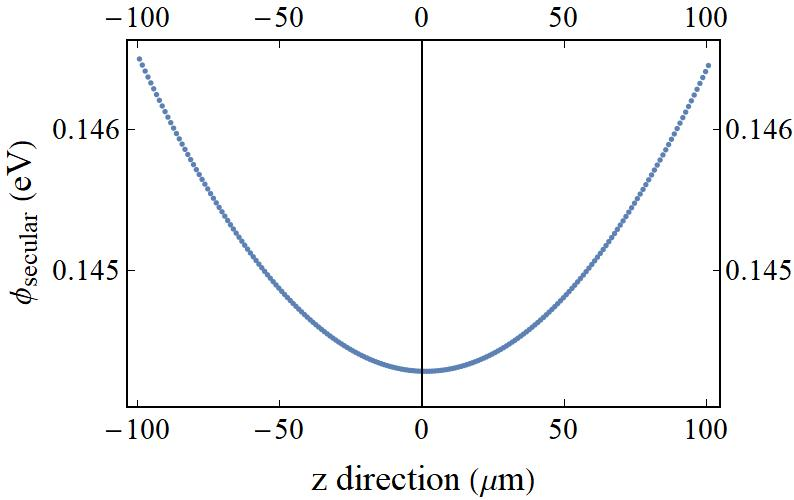
\includegraphics[width = 0.6\linewidth]{./simulation/figure/determine_SecFreq.jpg}
		\caption{Single-wellの条件にDouble-wellの条件におけるSecularポテンシャルのy方向の極小値におけるz軸に関するSecularポテンシャル(x=0)}
		\label{fig:determine_SecFreq}
	\end{center}
\end{figure}

\Eq{3D_harmonic}に示されるように,イオンの捕獲を行うポテンシャルは三次元の調和ポテンシャルとして記述されることから,\Fig{determine_SecFreq}で得られた曲線に二次関数によるフィッティングを施し,フィッティングパラメータから永年周波数が導かれる.x,y方向についても同様の計算が可能である.また,Double-wellの条件では,イオンが捕獲される2領域の一方の領域にフィッティングを施すことで,同様の計算を行うことができる.
